\newcommand{\dropperTagResultsAucTable}{
    \begin{table}[H]
        \centering
        \begin{tabular}{|p{2,8cm}||p{2,8cm} p{2,8cm} p{2,8cm}|}
            \hline
            Dropper Tag & ALOHA & Joint Embedding & Proposed Model \\
            \hline
            AUC-ROC & 0.972$\pm$0.001 & 0.972$\pm$0.001 & \textBF{0.976$\pm$0.002} \\
            \hline
        \end{tabular}
        \caption{AUC-ROC (Area Under Curve) of the different models for the \textbf{Dropper Tag} prediction task. Results were aggregated over \textBF{3} training runs with different weight initializations and minibatch orderings. Best results are shown in \textbf{bold}.} \label{tab:dropperTag_auc}
    \end{table}
}

\newcommand{\dropperTagResultsAtFprTable}{
    \begin{center}
        \begin{longtable}[c]{|p{3,2cm}||p{1,8cm} p{1,8cm} p{1,8cm} p{1,8cm} p{1,8cm}|}
            \hline
            Dropper Tag & \multicolumn{5}{c|}{{FPR}} \\
            & $10^{-5}$ & $10^{-4}$ & $10^{-3}$ & $10^{-2}$ & $10^{-1}$ \\
            \hline
            \endfirsthead

            \caption*{\raggedright ...continued from previous page} \\
            \hline
            Dropper Tag & \multicolumn{5}{c|}{\textbf{FPR}} \\
            & $10^{-5}$ & $10^{-4}$ & $10^{-3}$ & $10^{-2}$ & $10^{-1}$ \\
            \hline
            \endhead

            \caption*{\raggedleft ...continued on next page} \\
            \endfoot

            \caption{Mean and standard deviation results (TPR, Accuracy, Recall, Precision and F1-Score) of the different models for the \textbf{Dropper Tag} prediction task at different \textbf{FPR}s (\textit{False Positive Rates}). Results were aggregated over \textBF{3} training runs with different weight initializations and minibatch orderings. Best results are shown in \textbf{bold}. Under \textbf{TPR} results are also presented the percentage reduction in mean detection error and in ROC curve standard deviation introduced by the \textit{Proposed Model} with respect to both \textit{ALOHA} model and \textit{Joint Embedding}.} \label{tab:dropperTag_results_at_fpr} \\
            \endlastfoot

            \multicolumn{6}{|c|}{\textbf{TPR}} \\
            \hline
            ALOHA & 0.045$\pm$0.007 & 0.068$\pm$0.021 & 0.121$\pm$0.063 & 0.672$\pm$0.026 & 0.921$\pm$0.011 \\
            Joint Embedding & 0.064$\pm$0.018 & 0.092$\pm$0.028 & 0.142$\pm$0.020 & \textBF{0.682$\pm$0.011} & 0.922$\pm$0.008 \\
            Proposed Model & \textBF{0.079$\pm$0.023} & \textBF{0.121$\pm$0.032} & \textBF{0.245$\pm$0.083} & 0.674$\pm$0.063 & \textBF{0.936$\pm$0.005} \\
            \hline
            Error Reduction wrt \newline ALOHA & 3.6\% & 5.7\% & 14.1\% & 0.6\% & 19.0\% \\
            Error Reduction wrt \newline Joint Embedding & 1.6\% & 3.2\% & 12.0\% & -2.5\% & 17.9\% \\
            \hline
            Std Reduction wrt \newline ALOHA & -228.6\% & -52.4\% & -31.7\% & -142.3\% & 54.5\% \\
            Std Reduction wrt \newline Joint Embedding & -27.8\% & -14.3\% & -315.0\% & -472.7\% & 37.5\% \\
            \hline
            \multicolumn{6}{|c|}{\textbf{Accuracy}} \\
            \hline
            ALOHA & 0.878$\pm$0.001 & 0.881$\pm$0.003 & 0.887$\pm$0.008 & 0.949$\pm$0.003 & 0.903$\pm$0.001 \\
            Joint Embedding & 0.881$\pm$0.002 & 0.884$\pm$0.004 & 0.890$\pm$0.003 & \textBF{0.951$\pm$0.001} & 0.903$\pm$0.001 \\
            Proposed Model & \textBF{0.882$\pm$0.003} & \textBF{0.888$\pm$0.004} & \textBF{0.903$\pm$0.011} & 0.950$\pm$0.008 & \textBF{0.905$\pm$0.001} \\
            \hline
            \multicolumn{6}{|c|}{\textbf{Recall}} \\
            \hline
            ALOHA & 0.045$\pm$0.007 & 0.068$\pm$0.021 & 0.121$\pm$0.063 & 0.672$\pm$0.026 & 0.921$\pm$0.011 \\
            Joint Embedding & 0.064$\pm$0.018 & 0.092$\pm$0.028 & 0.142$\pm$0.020 & \textBF{0.682$\pm$0.011} & 0.922$\pm$0.008 \\
            Proposed Model & \textBF{0.079$\pm$0.023} & \textBF{0.121$\pm$0.032} & \textBF{0.245$\pm$0.083} & 0.674$\pm$0.063 & \textBF{0.936$\pm$0.005} \\
            \hline
            \multicolumn{6}{|c|}{\textbf{Precision}} \\
            \hline
            ALOHA & \textBF{0.999$\pm$0.000} & 0.989$\pm$0.004 & 0.931$\pm$0.035 & 0.908$\pm$0.003 & 0.574$\pm$0.003 \\
            Joint Embedding & \textBF{0.999$\pm$0.000} & 0.992$\pm$0.003 & 0.953$\pm$0.006 & \textBF{0.909$\pm$0.001} & 0.574$\pm$0.002 \\
            Proposed Model & \textBF{0.999$\pm$0.000} & \textBF{0.994$\pm$0.002} & \textBF{0.970$\pm$0.009} & 0.907$\pm$0.008 & \textBF{0.578$\pm$0.001} \\
            \hline
            \multicolumn{6}{|c|}{\textbf{F1 Score}} \\
            \hline
            ALOHA & 0.086$\pm$0.013 & 0.127$\pm$0.038 & 0.210$\pm$0.098 & 0.772$\pm$0.019 & 0.707$\pm$0.005 \\
            Joint Embedding & 0.120$\pm$0.031 & 0.166$\pm$0.047 & 0.246$\pm$0.031 & \textBF{0.779$\pm$0.008} & 0.708$\pm$0.004 \\
            Proposed Model & \textBF{0.145$\pm$0.040} & \textBF{0.214$\pm$0.051} & \textBF{0.385$\pm$0.105} & 0.772$\pm$0.045 & \textBF{0.715$\pm$0.003} \\
            \hline
        \end{longtable}
    \end{center}
}

\newcommand{\dropperTagResultsSummaryTable}{
    \begin{table}[H]
        \centering
        \begin{tabular}{|p{3,2cm}||p{1,8cm} p{1,8cm} p{1,8cm} p{1,8cm} p{1,8cm}|}
            \hline
            \multicolumn{6}{|c|}{Dropper Tag (at FPR $=1\%$)} \\
            \hline
            Model & TPR & Accuracy & Precision & Recall & F1 score \\
            \hline
            ALOHA & 0.672$\pm$0.026 & 0.949$\pm$0.003 & 0.908$\pm$0.003 & 0.672$\pm$0.026 & 0.772$\pm$0.019 \\
            Joint Embedding & \textBF{0.682$\pm$0.011} & \textBF{0.951$\pm$0.001} & \textBF{0.909$\pm$0.001} & \textBF{0.682$\pm$0.011} & \textBF{0.779$\pm$0.008} \\
            Proposed Model & 0.674$\pm$0.063 & 0.950$\pm$0.008 & 0.907$\pm$0.008 & 0.674$\pm$0.063 & 0.772$\pm$0.045 \\
            \hline
        \end{tabular}
        \caption{Summary of the mean and standard deviation results of the different models for the \textbf{Dropper Tag} prediction task at \textbf{FPR} $=1\%$. Results were aggregated over \textBF{3} training runs with different weight initializations and minibatch orderings. Best results are shown in \textbf{bold}.} \label{tab:dropperTag_result_summary}
    \end{table}
}

\newcommand{\dropperTagRocAloha}{
    \begin{figure}[H]
        \vspace*{-0.5cm}
        \centering
        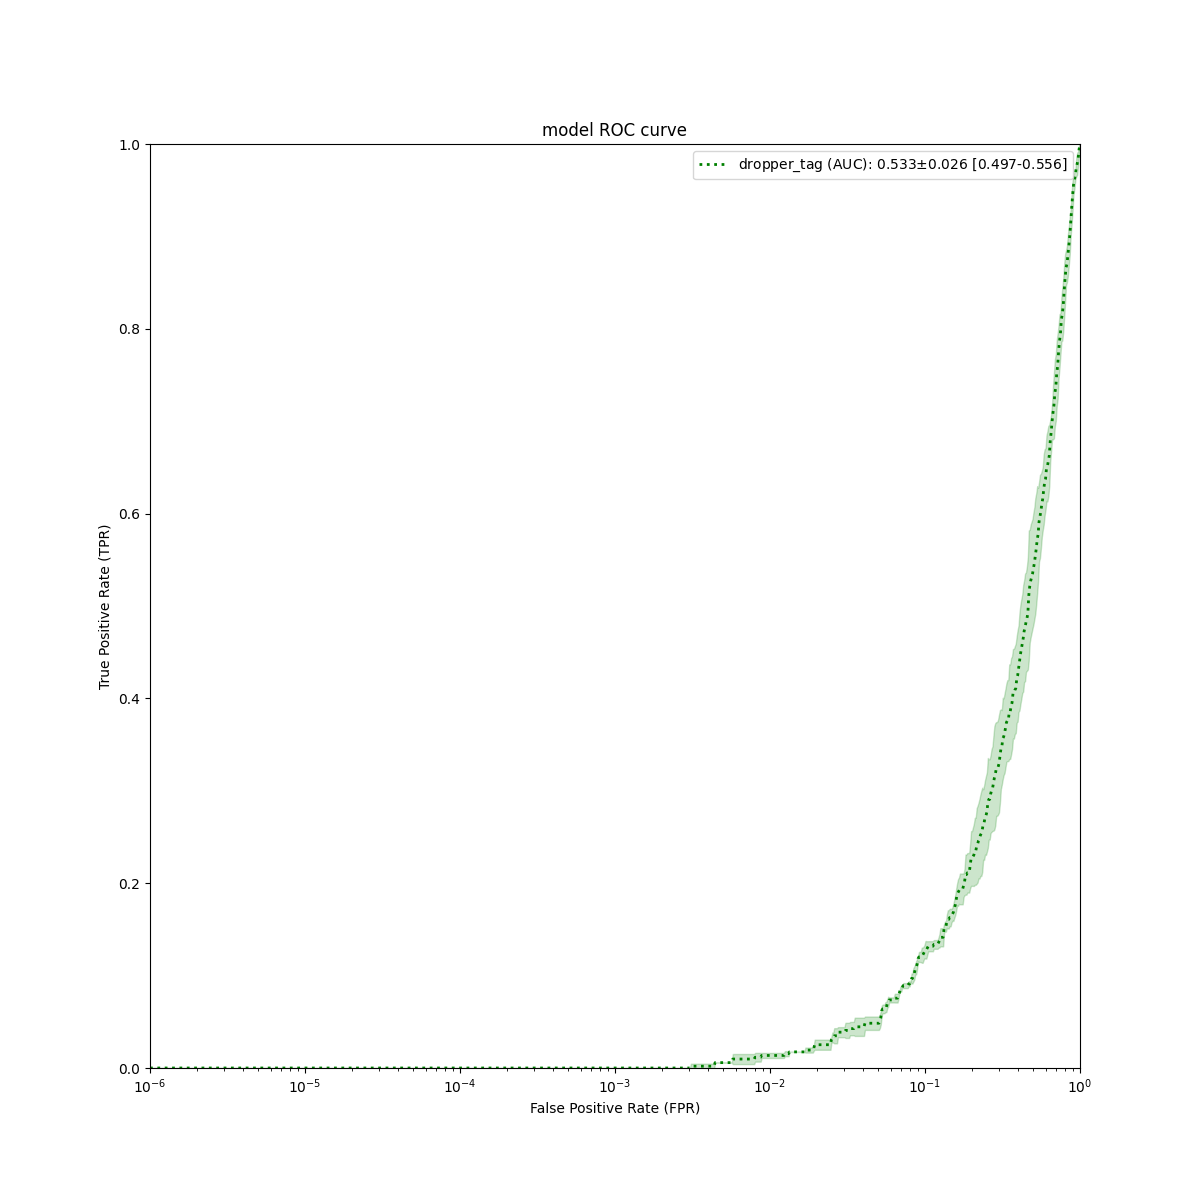
\includegraphics[width=0.6\textwidth]{./results/dropper_tag_roc_aloha.png}
        \vspace*{-0.2cm}
        \caption{ROC curve and AUC statistics of \textBF{ALOHA} model for the \textbf{Dropper Tag}. The line represents the \textit{mean} TPR at a given FPR, while the shaded region represents the \textit{standard deviation}. Statistics were computed over \textBF{3} training runs, each with random parameter initialization.}
        \label{fig:dropperTagRocAloha}
    \end{figure}
}

\newcommand{\dropperTagRocJointEmbedding}{
    \begin{figure}[H]
        \vspace*{-0.5cm}
        \centering
        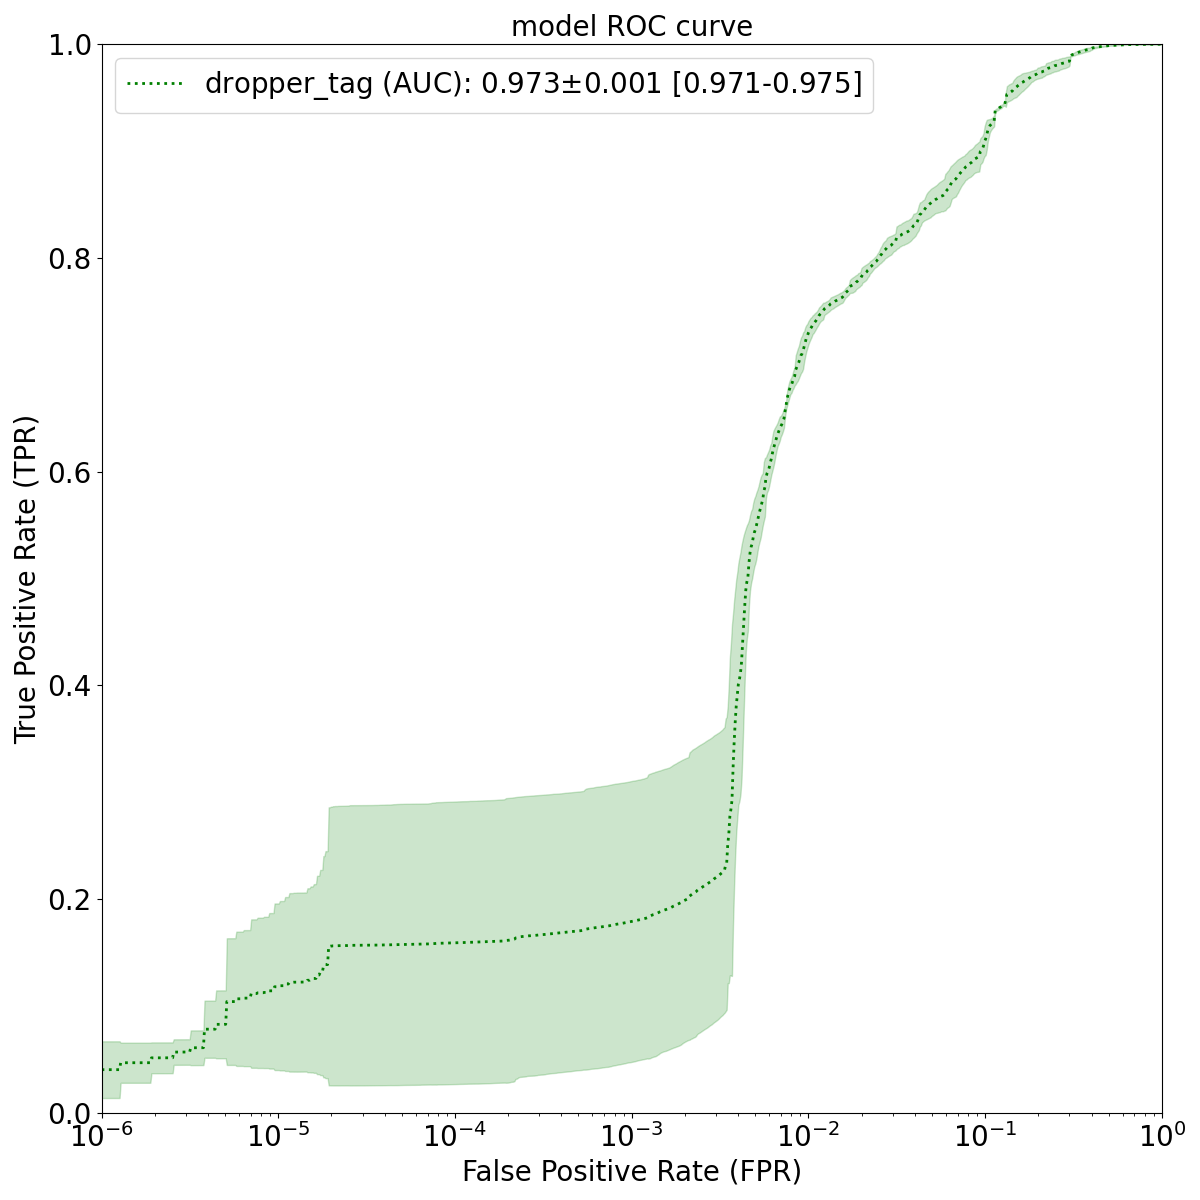
\includegraphics[width=0.6\textwidth]{./results/dropper_tag_roc_jointEmbedding.png}
        \vspace*{-0.2cm}
        \caption{ROC curve and AUC statistics of \textBF{Joint Embedding} model for the \textbf{Dropper Tag}. The line represents the \textit{mean} TPR at a given FPR, while the shaded region represents the \textit{standard deviation}. Statistics were computed over \textBF{3} training runs, each with random parameter initialization.}
        \label{fig:dropperTagRocJointEmbedding}
    \end{figure}
}

\newcommand{\dropperTagRocProposedMethod}{
    \begin{figure}[H]
        \vspace*{-0.5cm}
        \centering
        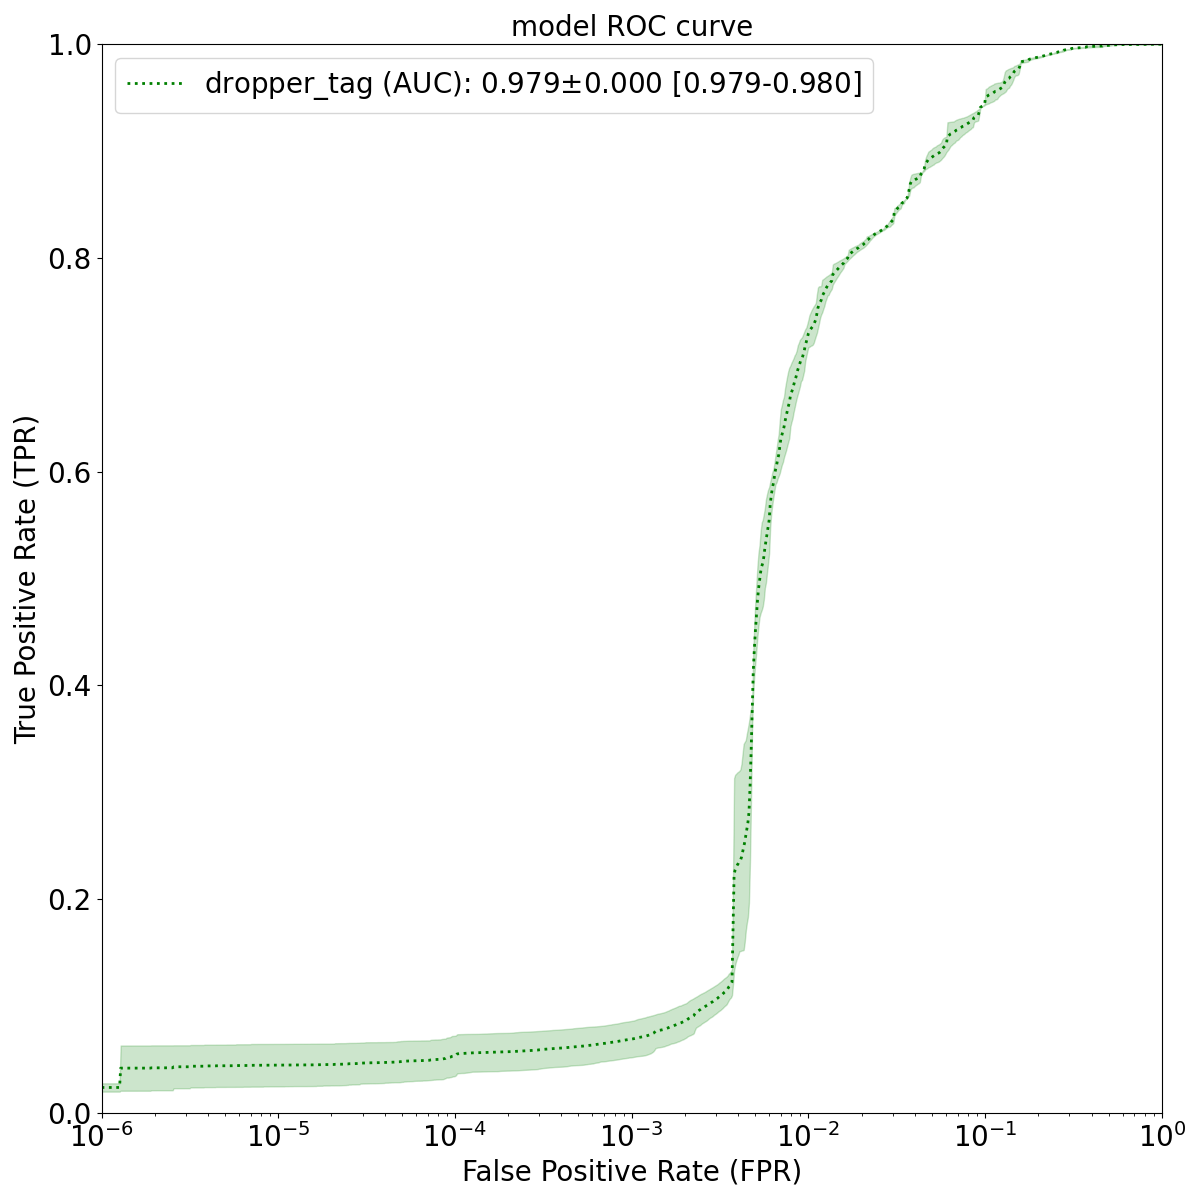
\includegraphics[width=0.6\textwidth]{./results/dropper_tag_roc_proposedModel.png}
        \vspace*{-0.2cm}
        \caption{ROC curve and AUC statistics of \textBF{Proposed Model} for the \textbf{Dropper Tag}. The line represents the \textit{mean} TPR at a given FPR, while the shaded region represents the \textit{standard deviation}. Statistics were computed over \textBF{3} training runs, each with random parameter initialization.}
        \label{fig:dropperTagRocProposedModel}
    \end{figure}
}
